%!TEX root = project.tex
\subsection{Uniform Disk}
\begin{figure}
    \centering
    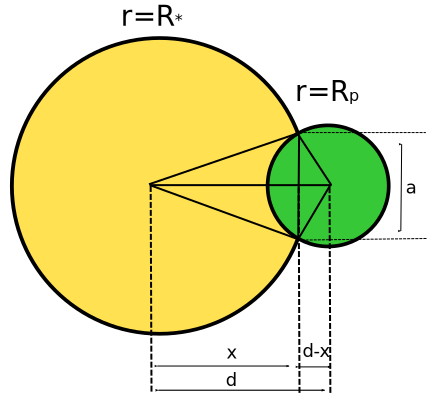
\includegraphics[width=\figwidth]{images/uniform_disk_overlap.pdf}
    \caption{Overlapping uniform disk model}
    \label{fig:uniform_overlap}
\end{figure}

A very simple model can be made by assuming that the transiting planet is a solid sphere with some radius $r_p$, that blocks all of the radiation from the star. Also, assume that the star itself, with radius $r_*$, emits radiation uniformly from all points, and that it too is a solid sphere.

In this model, there are three positions in the transit that need to be accounted for. Firstly, that the planet disk does not overlap the star, and no radiation is blocked. Secondly, that the planet's disk is fully contained within the disk of the star, and so the emitted radiation is blocked by the complete planetary disk. And thirdly that the disks overlap partially, and some factor less than during a complete overlap is blocked.

The amount of overlap of two circles of different size can be determined as follows:
\begin{align}
    A &= \kappa_1 + \kappa_2 - \kappa_3 \\
    \kappa_1 &= r_p^2\cos^{-1}\left(\frac{d^2 + r_p^2 - r_*^2}{2dr_p}\right)\\
    \kappa_2 &= r_*^2\cos^{-1}\left(\frac{d^2 + r_*^2 - r_p^2}{2dr_*}\right)\\
    \begin{split}
        \kappa_3 &= \frac{1}{2}\sqrt{(-d + r_p + r_*)}\sqrt{(d + r_p - r_*)}\times\\
        &\;\;\;\;\;\;\;\sqrt{(d - r_p + r_*)}\sqrt{(d + r_p + r_*)}
    \end{split}
\end{align}
While I arrived at this model independently, it is mathematically identical to the uniform disk model presented in \cite{mandel2002analytic}, although presented in a different form. An example transit using this model can be seen in figure \ref{fig:uniform_disk_model}. In each model I use a theoretical hot Jupiter, with parameters as shown in table \ref{tab:model}.
\begin{table}
\centering
\begin{tabular}{|l|r|}
\hline 
Parameter & Value \\
\hline
Star Radius & \RS \\
Star Mass &  \MS \\
Planet Radius & \RJ \\
Planet Mass & $2\MJ$ \\
Separation & $0.2\units{au}$ \\
\hline
\end{tabular}
\caption{Table of model parameters}
\label{tab:model}
\end{table}

\begin{figure}
    \centering
    \includegraphics[width=\figwidth]{images/uniform_disk_model.pdf}
    \caption{Expected observed flux from a transit as modelled as uniform disks}
    \label{fig:uniform_disk_model}
\end{figure}

\subsection{Limb Darkening}
\begin{figure}
    \centering
    \includegraphics[width=\figwidth]{images/venus_transit.jpg}
    \caption{Image of the Sun taken during the 2012 Venus Transit, provided courtesy of Brocken Inaglory}
    \label{fig:limb_darkening_image}
\end{figure}

While the uniform disk model is a good approximation, it is not an accurate description of what is observed. Stars appear to in fact have a decreasing intensity towards the outer edge than in the center. This limb darkening is due to two effects. Both the temperature and density of the star decrease as a function of radius. This can be seen clearly in figure \ref{fig:limb_darkening_image}.
\begin{figure}
    \centering
    \includegraphics[width=\figwidth]{images/model_comparison.pdf}
    \caption{Comparison of Uniform disk and quadratic limb-darkening models}
    \label{fig:model_comparison}
\end{figure}

A comparison between transits as predicted by both the simple uniform disk model, and an example model which includes limb-darkening can be seen in figure \ref{fig:model_comparison}.
